\documentclass[a4paper, 14pt]{extarticle}

% Поля
%--------------------------------------
\usepackage{geometry}
\geometry{a4paper,tmargin=2cm,bmargin=2cm,lmargin=3cm,rmargin=1cm}
%--------------------------------------


%Russian-specific packages
%--------------------------------------
\usepackage[T2A]{fontenc}
\usepackage[utf8]{inputenc} 
\usepackage[english, main=russian]{babel}
%--------------------------------------

\usepackage{textcomp}

% Красная строка
%--------------------------------------
\usepackage{indentfirst}               
%--------------------------------------             


%Graphics
%--------------------------------------
\usepackage{graphicx}
\graphicspath{ {./images/} }
\usepackage{wrapfig}
%--------------------------------------

% Полуторный интервал
%--------------------------------------
\linespread{1.3}                    
%--------------------------------------

%Выравнивание и переносы
%--------------------------------------
% Избавляемся от переполнений
\sloppy
% Запрещаем разрыв страницы после первой строки абзаца
\clubpenalty=10000
% Запрещаем разрыв страницы после последней строки абзаца
\widowpenalty=10000
%--------------------------------------

%Списки
\usepackage{enumitem}

%Подписи
\usepackage{caption} 

%Гиперссылки
\usepackage{hyperref}

\hypersetup {
	unicode=true
}

%Рисунки
%--------------------------------------
\DeclareCaptionLabelSeparator*{emdash}{~--- }
\captionsetup[figure]{labelsep=emdash,font=onehalfspacing,position=bottom}
%--------------------------------------

\usepackage{tempora}

%Листинги
%--------------------------------------
\usepackage{listings}
\lstset{
  basicstyle=\ttfamily\footnotesize, 
  %basicstyle=\footnotesize\AnkaCoder,        % the size of the fonts that are used for the code
  breakatwhitespace=false,         % sets if automatic breaks shoulbd only happen at whitespace
  breaklines=true,                 % sets automatic line breaking
  captionpos=t,                    % sets the caption-position to bottom
  inputencoding=utf8,
  frame=single,                    % adds a frame around the code
  keepspaces=true,                 % keeps spaces in text, useful for keeping indentation of code (possibly needs columns=flexible)
  keywordstyle=\bf,       % keyword style
  numbers=left,                    % where to put the line-numbers; possible values are (none, left, right)
  numbersep=5pt,                   % how far the line-numbers are from the code
  xleftmargin=25pt,
  xrightmargin=25pt,
  showspaces=false,                % show spaces everywhere adding particular underscores; it overrides 'showstringspaces'
  showstringspaces=false,          % underline spaces within strings only
  showtabs=false,                  % show tabs within strings adding particular underscores
  stepnumber=1,                    % the step between two line-numbers. If it's 1, each line will be numbered
  tabsize=2,                       % sets default tabsize to 8 spaces
  title=\lstname                   % show the filename of files included with \lstinputlisting; also try caption instead of title
}
%--------------------------------------

%%% Математические пакеты %%%
%--------------------------------------
\usepackage{amsthm,amsfonts,amsmath,amssymb,amscd}  % Математические дополнения от AMS
\usepackage{mathtools}                              % Добавляет окружение multlined
\usepackage[perpage]{footmisc}
%--------------------------------------

%--------------------------------------
%			НАЧАЛО ДОКУМЕНТА
%--------------------------------------

\begin{document}

%--------------------------------------
%			ТИТУЛЬНЫЙ ЛИСТ
%--------------------------------------
\begin{titlepage}
\thispagestyle{empty}
\newpage


%Шапка титульного листа
%--------------------------------------
\vspace*{-60pt}
\hspace{-65pt}
\begin{minipage}{0.3\textwidth}
\hspace*{-20pt}\centering

\includegraphics[width=\textwidth]{emblem}
\end{minipage}
\begin{minipage}{0.67\textwidth}\small \textbf{
\vspace*{-0.7ex}
\hspace*{-6pt}\centerline{Министерство науки и высшего образования Российской Федерации}
\vspace*{-0.7ex}
\centerline{Федеральное государственное бюджетное образовательное учреждение }
\vspace*{-0.7ex}
\centerline{высшего образования}
\vspace*{-0.7ex}
\centerline{<<Московский государственный технический университет}
\vspace*{-0.7ex}
\centerline{имени Н.Э. Баумана}
\vspace*{-0.7ex}
\centerline{(национальный исследовательский университет)>>}
\vspace*{-0.7ex}
\centerline{(МГТУ им. Н.Э. Баумана)}}
\end{minipage}
%--------------------------------------

%Полосы
%--------------------------------------
\vspace{-25pt}
\hspace{-35pt}\rule{\textwidth}{2.3pt}

\vspace*{-20.3pt}
\hspace{-35pt}\rule{\textwidth}{0.4pt}
%--------------------------------------

\vspace{1.5ex}
\hspace{-35pt} \noindent \small ФАКУЛЬТЕТ\hspace{80pt} <<Информатика и системы управления>>

\vspace*{-16pt}
\hspace{47pt}\rule{0.83\textwidth}{0.4pt}

\vspace{0.5ex}
\hspace{-35pt} \noindent \small КАФЕДРА\hspace{50pt} <<Теоретическая информатика и компьютерные технологии>>

\vspace*{-16pt}
\hspace{30pt}\rule{0.866\textwidth}{0.4pt}
  
\vspace{11em}

\begin{center}
\Large {\bf Лабораторная работа № 4.2} \\
\large {\bf по курсу <<Численные методы линейной алгебры>>} \\
\large <<Вычисление собственных значений и собственных
векторов матрицы методом А. Н. Крылова>>
\end{center}\normalsize

\vspace{8em}


\begin{flushright}
  {Студентка группы ИУ9-72Б Самохвалова П. С. \hspace*{15pt}\\
  \vspace{2ex}
  Преподаватель Посевин Д. П.\hspace*{15pt}}
\end{flushright}

\bigskip

\vfill
 

\begin{center}
\textsl{Москва 2023}
\end{center}
\end{titlepage}
%--------------------------------------
%		КОНЕЦ ТИТУЛЬНОГО ЛИСТА
%--------------------------------------

\renewcommand{\ttdefault}{pcr}

\setlength{\tabcolsep}{3pt}
\newpage
\setcounter{page}{2}

\section{Цель работы}\label{Sect::goal}

Реализовать вычисление собственных значений и собственных
векторов матрицы методом А. Н. Крылова.

\section{Задание}\label{Sect::task}

\begin{itemize}
    \item Найти собственные значения и собственные векторы матрицы методом А. Н. Крылова.
    \item Сравнить результаты с методом А. М. Данилевского.
\end{itemize}

\section{Практическая реализация}\label{Sect::code}

Исходный код программы представлен в листинге~\ref{lst:code1}.

\begin{lstlisting}[language={python},caption={Вычисление собственных значений и собственных векторов матрицы методом А. Н. Крылова},label={lst:code1}]
from num_methods import *
import random
import copy


def krylov_method(a):
    n = len(a)
    y = [[0] * n for i in range(n + 1)]
    y[0][0] = 1
    for i in range(1, n + 1):
        y[i] = mult_matr_vec(a, y[i - 1])
    m = [[1] * n for i in range(n)]
    for i in range(n):
        for j in range(n):
            m[i][j] = y[n - 1 - j][i]
    p = gauss_method(m, y[n])
    g = gershgorin_rounds(a)
    ls = div_half_method(g[0], g[1], func(p))
    p = p[::-1]
    q = [[0] * n for i in range(n)]
    for i in range(n):
        for j in range(n):
            if j == 0:
                q[j][i] = 1
            else:
                q[j][i] = ls[i] * q[j - 1][i] - p[n - j]
    x = []
    for i in range(n):
        xi = [0] * n
        for j in range(n):
            xi = sum_vec(xi, mult_vec_num(q[j][i], y[n - 1 - j]))
        x.append(xi)
    return ls, x


a = [[2.2, 1, 0.5, 2],
     [1, 1.3, 2, 1],
     [0.5, 2, 0.5, 1.6],
     [2, 1, 1.6, 2]]
n = len(a)
print("Krylov method for matrix 4x4")
ls, x = krylov_method(a)
print("Eigenvalues of matrix")
print(ls)
print("Eigenvectors of matrix")
for xi in x:
    norm = norm_vec(xi)
    for i in range(n):
        xi[i] /= norm
    print(xi)
print()
print("Krylov method for matrix 7x7")
a = generate_symm_matrix(7, -10, 10)
n = len(a)
ls, x = krylov_method(a)
print("Eigenvalues of matrix")
print(ls)
print("Eigenvectors of matrix")
for xi in x:
    norm = norm_vec(xi)
    for i in range(n):
        xi[i] /= norm
    print(xi)
print()
print("Danilevsky method for matrix 7x7")
d, b = danilevsky_method(a)
p = d[0][:]
g = gershgorin_rounds(a)
ls = div_half_method(g[0], g[1], func(p))
print("Eigenvalues of matrix")
print(ls)
print("Eigenvectors of matrix")
vectors = []
for l in ls:
    y = [1]
    for i in range(1, n):
        y.append(l ** i)
    y = y[::-1]
    y = mult_matr_vec(b, y)
    norm = norm_vec(y)
    for i in range(n):
        y[i] /= norm
    vectors.append(y)
    print(y)
\end{lstlisting}

\section{Результаты}\label{Sect::res}

Результаты работы программы представлены на рисунках~\ref{fig:img1}~--~\ref{fig:img3}. 

\begin{figure}[!htb]
	\centering
	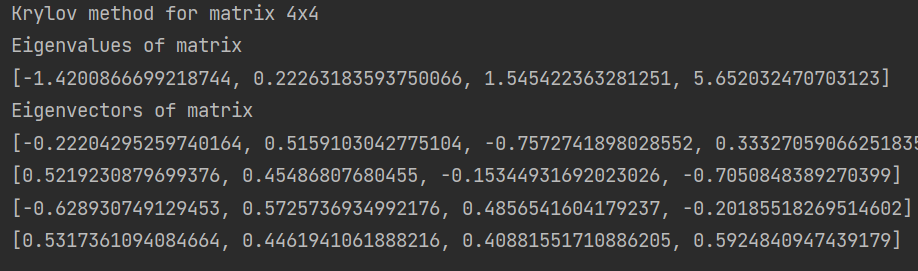
\includegraphics[width=0.8\textwidth]{img1}
\caption{Собственные значения и собственные векторы матрицы 4х4 методом А. Н. Крылова}
\label{fig:img1}
\end{figure}

\begin{figure}[!htb]
	\centering
	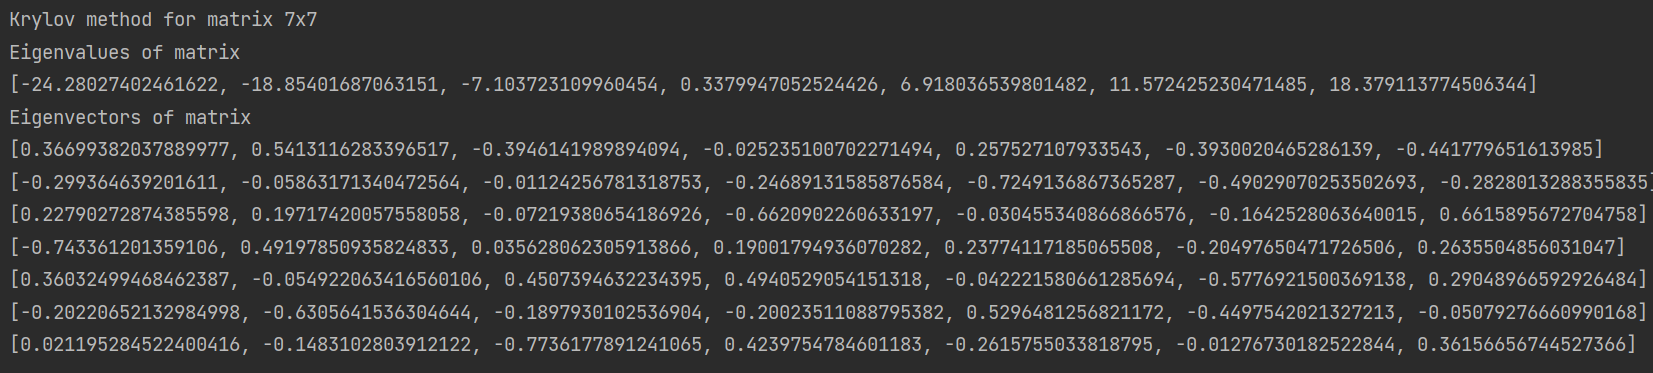
\includegraphics[width=0.8\textwidth]{img2}
\caption{Собственные значения и собственные векторы матрицы 7х7 методом А. Н. Крылова}
\label{fig:img2}
\end{figure}

\begin{figure}[!htb]
	\centering
	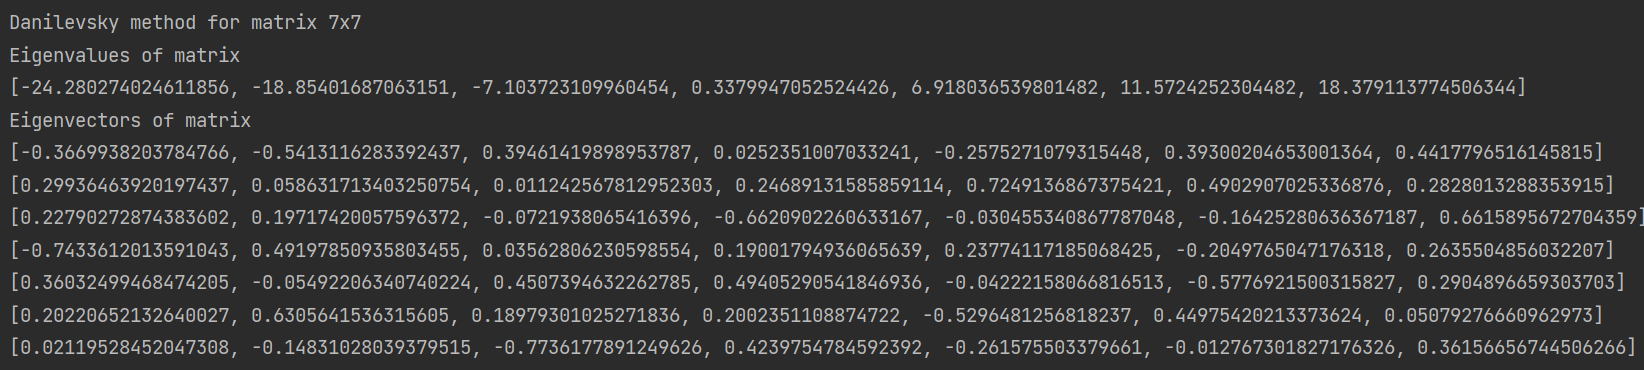
\includegraphics[width=0.8\textwidth]{img3}
\caption{Собственные значения и собственные векторы матрицы 7х7 методом А. М. Данилевского}
\label{fig:img3}
\end{figure}

\section{Выводы}\label{Sect::conclusion}

В результате выполнения лабораторной работы было реализовано вычисление собственных значений и собственных векторов матрицы методом А. Н. Крылова.
\end{document}
